\subsection{Hypothesis Algorithm}%
\label{subsec:halgorithm}
This section first discusses the search and execution loop that reside in the proposed \ac{halgorithm}. Then termology is eleborated upon to understand the pseudocode and flowchart of the proposed \ac{halgorithm}. This section finalises with 4 examples.\bs

\paragraph{Initialisation of the \ac{halgorithm}}
The \ac{halgorithm} is initialised with a task, consisting of subtasks. For every subtask a start and target node are created and their status is set to Initialized. Then the goal of the \ac{halgorithm} is to connect the every starting node to its corresponding target node with an hypothesis. When an hypothesis is completed succesfully, the target node's status is set to Completed. If the \ac{halgorithm} was unable to find an hypothesis that completes a subtask, the \ac{halgorithm} concludes it cannot complete that subtask, and the target node's status is set to Failed.\bs


\paragraph{The Search and the Execution Loop}
The proposed algorithm is composed by two main parts, a search loop and an execution loop. In the search loop the \ac{halgorithm} searches for hypothesis, in the executions loop the \ac{halgorithm} tests hypotheses by executing the edges which form the hypothesis. Later in this chapter a flowchart is discussed, in \Cref{tikz:flowchart_hgraph}, here the two main loops can be identified, see \Cref{fig:two_loops_identified}.\bs
\begin{figure}[H]
    \centering
    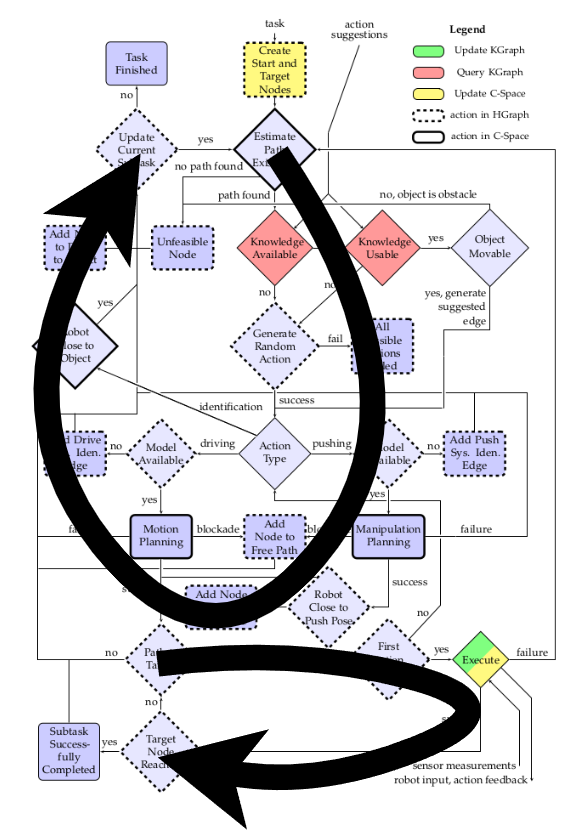
\includegraphics[width=7cm]{figures/proposed_method/two_loops_identified}
    \caption{The search (above) and execution (below) loop, that make up the two main parts of the proposed \ac{halgorithm}.}%
    \label{fig:two_loops_identified}
\end{figure}



\paragraph{Finding unfinished subtasks}
Whilst the \ac{halgorithm} resides in the search loop, hypotheses are formed. Forming a hypothesis generates nodes, edges, and progressing their status as described in \Cref{tikz:status_identification_edge,tikz:status_action_edge}. In the execution loop \textit{an edge is being executed}, a phrase to describe that the controller residing in an edge is sending control input toward the robot. The \ac{halgorithm} operates synchronously. The result is that the robots cannot operate whilst the \ac{halgorithm} resides in the search loop, and during execution, no hypothesis can be formed or updated. The \ac{halgorithm} alternates between seach and execution loop, when in the search loop an hypothesis is generated, that hypothesis is tested in the execution loop. The execution loop executes the edges that form the hypothesis one by one, untill either a fault is detected or the hypothesis is completed. Upon fault or completion, the \ac{halgorithm} alternates back to the search loop\bs

\paragraph{Creating an hypothesis for a subtask}
If the \textit{SubTaskNotFinished} returns an unfinished subtask, the \ac{halgorithm} starts searching for an hypothesis that can connect the start node to the corresponding target node.
When entering or re-entering the search loop, the first thing to determine is if there are unfinished subtasks, and if unfinished subtasks exists, which nodes to connected in order to form a hypothesis that completes that subtask. For such functionality three functions are created; \textit{SubTaskNotFinished}, \textit{goBackward(\gls{node})}, \textit{findCorrespondingNode(\gls{node})}. These functions are now discussed.\bs

First, determining if there exist a unfinished subtask with the \textit{SubTaskNotFinished(\gls{subtask})} function. It checks the status for every target node in \ac{hgraph}. The three status (Initialised, Completed, Failed) and selects a target node with an Initialised status that corresponds to a uncompleted subtask. If all existing target nodes have either a Completed or Failed status, the \ac{halgorithm} concludes that the task is completed.\bs

 The \ac{halgorithm} relies on a backward search technique. The backward search technique can be described as: \textit{start the search at a goal state and work backward until the initial state is encountered~\cite{lavalle_planning_2006}.} A motivation for a backward search over a forward search is that, it might be the case that the branching factor is large when starting from the initial state. In such cases, it might be more efficient to use a backward search. If the \textit{SubTaskNotFinished} returns an unfinished subtask, the \ac{halgorithm} starts searching for an hypothesis that can connect the start node to the corresponding target node. The first step is to find the right nodes in the \ac{hgraph} which is now discussed.\bs

 The \textit{goBackward($\gls{node}_\mathit{target}$)} function takes the a target node $\gls{node}_target$ that corresponds to a unfinised subtask. It then traverses backwards via non-failed edges to find the node that points toward the target node. The function stops traversing back when it encountered a node with a Failed status, or when there exist no edge to traverse over. It returns the last node, that node points toward the target node over a sequence of edges with a status other than Failed and all point toward nodes with a status other than Failed.\bs

The \textit{goBackward($\gls{node}_\mathit{target}$)} finds a node to connect toward, now a corresponding node is sought to connect from, with the \textit{findCorrespondingNode(\gls{node})} to later create an edge connecting both nodes. It takes a paremeter the node to connect toward, \textit{findCorrespondingNode(GoBackward($\gls{node}_\mathit{target}$))} has returns an existing node that has the same contains the same object as GoBackward($\gls{node}_\mathit{target}$), if such a node does not exist, it is created.

When the \ac{hgraph} only contains start and target nodes, the \textit{GoBackward($\gls{node}_\mathit{target}$)} will return $\gls{node}_\mathit{target}$ and \textit{findCorrespondingNode(GoBackward($\gls{node}_\mathit{target}$))} will return $\gls{node}_\mathit{start}$.\bs

Both nodes are renamed to prevent long function names, $\gls{node}_\mathit{to} =  \mathit{GoBackward(\gls{node}_\mathit{target})}, \gls{node}_\mathit{from} = \mathit{findCorrespondingNode(GoBackward(\gls{node}_\mathit{target}))}$.\bs

\paragraph{Creating Edges}
The \textit{connectWithEdge($\gls{node}_1, \gls{node}_2$)} function connects two nodes with an edge, such a the nodes $\gls{node}_\mathit{from}, \gls{node}_\mathit{to}$ just introduced. In this thesis the robot can take two actions, drive and push. To detrmine the action edge to connect the two nodes, both objects that are containted by both nodes must be equal. Do both nodes contain the robot as object, create a drive action edge, do both nodes contain an object other than the robot, create a push action edge.\bs


\paragraph{Completing an Hypothesis}
a valid hypothesis in the \ac{hgraph} must start at the robot node, containt the start node and point toward the target node. thus a driving subtask, where the target node contains the robot object, start at the robot node, and points toward the target node. for a pushing subtask, where the target node contains an object, a valid hypothesis start at the robot node, points toward the start node that contains the object, and points toward the target node that contains the object.\bs

to check if an hypothesis is valid the \textit{isconnected($\gls{node}_1, \gls{node}_2$)} is created. this function checks if there exist a path in the \ac{hgraph} from $\gls{node}_1$ to $\gls{node}_2$ over a sequence of edges with a status other than failed.

checking if a hypothesis is valid depents on the object in the target node.

an hypothesis is valid if:

the target node contains the robot object $\gls{obj}_\textit{robot-target}$ and \textit{isconnected($\gls{node}_\mathit{robot-start}, \gls{node}_\mathit{robot-target}$)} evaluates to true.
the target node contains object $\gls{obj}_\textit{id}$ and \textit{isconnected($\gls{node}_\mathit{robot}, \gls{node}_\mathit{obj-start}$)}, \textit{isconnected($\gls{node}_\mathit{obj-start}, \gls{node}_\mathit{obj-target}$)} both evaluate to true.

\paragraph{Preparing edges for Execution}
A valid hypothesis is not yet an hypothesis ready to be executed. For example, an initialised edge does not yet have a path to track. 

\todo{push edges make an extra node for the robot, connect that }
\textit{ReadyForExecution(\gls{edge})}:
\textit{MakeReady(\gls{edge})}:


\paragraph{Hypothesis Execution}

\textit{incrementEdge}:
\textit{SteerTowardTarget(\gls{observation})}:
\textit{TargetNotReached(\gls{edge})}:


\paragraph{Fault Detection}

\textit{FaultDetected(\gls{edge})}:

\textit{HandleFault(\gls{edge})}:

\todo{Corrado: SOmewhere here must be an equetion that if eveolves to true, determines if a subtask was completed}




\noindent
\begin{algorithm}[H]
  \caption{Pseudocode for the proposed hypothesis algorithm.}\label{pseudocode:halgorithm}
  \begin{algorithmic}[1]

    \hspace{-0.9cm}\colorbox{my_grey}{\parbox{\linewidth}{%
        \For{$\gls{subtask} \in \gls{task}$}

        \hspace{-0.1cm}\colorbox{my_yellow}{\parbox{\linewidth}{%
            \While{\textit{SubTaskNotFinished(\gls{subtask})}}\algorithmiccomment{Search Loop}
            \If{\textit{\gls{hgraph}.isConnected(\gls{subtask}.start, \gls{subtask}.target)}}
            \If{\textit{\gls{hypothesis}.currentEdge.readyForExecution}}

            \hspace{-0.1cm}\colorbox{my_light_blue}{\parbox{\linewidth}{%
                \While{\textit{TargetNotReached(\gls{hypothesis}.currentEdge)}} \algorithmiccomment{Execution Loop}
                \If{\textit{FaultDetected(\gls{hypothesis}.currentEdge)}}
                \State \textit{HandleFault(\gls{hypothesis}.currentEdge)}
                \State break
                \EndIf
                \State \textit{\gls{hypothesis}.currentEdge.steerTowardTarget(\gls{observation})}
                \If{\textit{TargetReached(\gls{hypothesis}.currentEdge)}}
                \If{\textit{readyForExecution(\gls{hypothesis}.currentEdge)}}
                  \State \textit{\gls{hypothesis}.incrementEdge}
                \Else
                  \State break
                \EndIf
                \EndIf
                \EndWhile
            }}
            \Else
            \State \textit{makeReady(\gls{hypothesis}.currentEdge)}
            \EndIf
            \Else
            \State $\mathit{\gls{node}_{localtarget}} \leftarrow \gls{hgraph}.\mathit{goBackward(\gls{node}.target)}$
            \State $\mathit{\gls{node}_{localstart}} \leftarrow \gls{hgraph}.\mathit{findCorrespondingNode(\gls{node}_{localtarget})}$
            \State $\mathit{G.connectWithEdge}(\gls{node}_\mathit{localstart}, \gls{node}_\mathit{localtarget})$
            \EndIf
            \EndWhile
        }}
        \EndFor
    }}
  \end{algorithmic}
\end{algorithm}

During a backward search, edges are added pointing toward the target node (or to nodes that point toward the target node). Trying to connect the robot node through a list of successive directed edges to a target node. If such a path has been found in the \ac{hgraph}, a hypothesis has been found and the robot can start executing edges.\bs


A flowchart of the \ac{halgorithm} is presented in \Cref{tikz:flowchart_hgraph}. Compared to the mathematical description of the \ac{halgorithm} the flowchart provides more detail, including an elaborate description for every block in the flowchart (see \Cref{table:explainer_hgraph_figures_nodes}). The flowchart includes path estimation, planning and the behavior when failure occurs. A connection point to the \ac{kgraph} and robot environment are included. The blocks in the flowchart indicate which action they take and where, such as the configuration space, the \ac{kgraph} or the \ac{hgraph}. \todo{Corrado: rephrase what is below:}
With the flowchart is straightforward to see how the \ac{halgorithm} connects to the status of edges, with the mathematical description of the \ac{halgorithm} that is harder so see. Compared to the flowchart the mathematical description is a abstracted version, leaving many details out that are related to the robot in this thesis. An abstracted mathematical description is simpler and encompasses a broader field of robots. So could the mathematical description also be applied to another robot such as a movable robot with robot arm and gripper. The flowchart encompasses to many details to be applied after such an change in robot hardware.

% \newgeometry{left=1.1cm,bottom=0.1cm,top=1.9cm,headsep=0.1in,heightrounded}

\newpage
\vspace*{-1.2cm}
\hspace{-1.2cm}
\begin{minipage}{10cm}
\begin{figure}[H] 
\centering
\begin{tikzpicture}]
  [node distance = 3cm] 

    % Nodes
    \node [block, fill=yellow!50, line width=2pt, dashed] (first) {Create Start and Target Nodes};
    
    % legend
    \node[text width=2.8cm, yshift=0.6cm, right of=first, node distance=7cm, text centered, rounded corners, minimum height=1em, label={[name=lab, yshift=0.4cm, left]\textbf{Legend}}] (legend1) {\small Update KGraph};
    \node[rectangle, draw, left of=legend1, fill=green!50, rounded corners, minimum height=1em, minimum width=1cm, node distance=2cm] (legend1color) {};
    
    \node[text width=2.8cm, below of=legend1, text centered, minimum height=1em, node distance=0.7cm] (legend2) {\small Query KGraph};
    \node[rectangle, draw, left of=legend2, fill=red!40, rounded corners, minimum height=1em, minimum width=1cm, node distance=2cm] (legend2color) {};
   
    \node[text width=2.8cm, below of=legend2, text centered, minimum height=1em, node distance=0.7cm] (legend3) {\small Update C-Space};
\node[rectangle, draw, left of=legend3, fill=yellow!50, rounded corners, minimum height=1em, minimum width=1cm, node distance=2cm] (legend3color) {};
    
    \node[text width=2.8cm, below of=legend3, text centered, minimum height=1em, node distance=0.7cm] (legend4) {\small action in HGraph};
    \node[rectangle, draw, left of=legend4, rounded corners, minimum height=1em, minimum width=1cm, node distance=2cm, line width=2pt, dashed] (legend4color) {};
 
    \node[text width=2.8cm, below of=legend4, text centered, minimum height=1em, node distance=0.7cm] (legend5) {\small action in C-Space};
\node[rectangle, draw, left of=legend5, rounded corners, minimum height=1em, minimum width=1cm, node distance=2cm, line width=2pt] (legend5color) {};

    % nodes, Path exists 
    \node [decision, below of=first, node distance=2.6cm, line width=2pt] (path_existence) {Estimate Path Existence};
    \node [decision, left of=path_existence, node distance=4.5cm, line width=2pt, dashed] (subtasks) {Is There an Unfinished Subtask};

    \node [block, above of=subtasks, node distance=2.8cm] (no_solution_found) {Task Finished};
    
    % nodes, Knowledge available
    \node [decision, fill=red!40, below of=path_existence, node distance=3.2cm, inner sep=0.5mm] (know_avail) { Knowledge Available };
    \node [decision, fill=red!40, right of=know_avail, node distance=3.5cm, inner sep=0.5mm] (know_good) {Knowledge Usable};
    \node [decision, right of=know_good, node distance=3.5cm, text width=1.7cm] (movable) {\vspace{0.1cm}\shortstack[]{Object\\Movable or\\Unknown}};
    \node [block, left of=know_avail, node distance=3cm, line width=2pt, dashed] (impossible) {Impossible Node};
    
    % nodes, Generate new edge
    \node [decision, below of=know_avail, node distance=3.2cm, line width=2pt, inner sep=0.5mm, dashed] (goto_sys_iden) {Generate Random Action};

    \node[block, right of=goto_sys_iden, node distance=3.5cm, line width=2pt, dashed] (no_trans_found) {All Possible Actions Failed};
    
    
    % Motion/Manipulation planning 
    \node [decision, below of=goto_sys_iden, node distance=3.5cm] (single_multi) {Action Type};

    \node [decision, line width=2pt, dashed, left of=single_multi, node distance=3.7cm] (model_avail_single) {Model Available};
    \node [decision, line width=2pt, dashed, right of=single_multi, node distance=3.7cm] (model_avail_multi) {Model Available};
    \node [block, line width=2pt, dashed, left of=model_avail_single, node distance=2.8cm] (sys_iden_single) {Add Drive Sys. Iden. Node};
    \node [block, line width=2pt, dashed, right of=model_avail_multi, node distance=2.8cm] (sys_iden_multi) {Add Push Sys. Iden. Node};
    \node [block, line width=2pt, dashed, below of=single_multi, node distance=2.7cm] (move_object) {Add Node to Move Object};
    \node [block, line width=2pt, left of=move_object, node distance=3.7cm] (motion_planning) {Motion Planning};
    \node [block, line width=2pt, right of=move_object, node distance=3.7cm, text width=2.1cm] (manipulation_planning) {Manipulation Planning};

    \node [decision, line width=2pt, dashed, minimum width=2.3cm, below of=move_object, node distance=2.3cm, xshift=1.75cm] (drive_to_push_position) {Robot Close to Push Pose};
    \node [block, line width=2pt, dashed, minimum width=2.3cm, below of=move_object, node distance=2.3cm, xshift=-1.75cm] (goto_push_position) {Add Node to Drive to Push Pose};
  
    \node [decision, line width=2pt, above of=sys_iden_single, node distance=3.5cm] (add_drive_node) {Robot Close to Object};

    \node [block, dashed, line width=2pt, above of=add_drive_node, node distance=3.2cm] (do_add_drive_node) {Add Node to Drive to Object};

    % nodes, Path to target
    \node [decision, below of=motion_planning, node distance=4.0cm, line width=2pt, dashed] (global_path) {Path to Target}; 
1   \node [decision, right of=global_path, node distance=7.4cm, line width=2pt, dashed] (first_action) {First Action Planned};

    \node [decision, right of=first_action, diagonal fill={yellow!50}{green!50}, node distance=3cm] (execute) {Execute};
     
    % nodes, Target node reached 
    \node [decision, below of=global_path, node distance=3cm, line width=2pt, dashed] (target_node_reached) {Target Node Reached};
    \node [block, left of=target_node_reached, node distance=3cm] (end) {Subtask Successfully Completed};
    
    % Edges
    \path[line] ++(0,1.2) -- node[yshift=0.2cm, above]{task} (first);
    \path[line] (first) -- node[midway](to_path_exists){}(path_existence); 
    
    % edges, Path exists 
    \path[line] ([xshift=0.2cm, yshift=-0.2cm] path_existence.south west) -| node[near start, xshift=-0.4cm, above] {no path found} (impossible.north);
    \path[line] (subtasks.north) --  node[left] {no} (no_solution_found);
    \path[line] (path_existence) -- node[xshift=0cm, yshift=0.15cm, left] {path found} (know_avail); 
    \path[line] (subtasks.east) -- node[above] {yes} (path_existence.west);
    
    % edges, Knowledge available
    \path[line] (know_avail) -- node[above] {yes} (know_good); 
    \path[line] (know_good) -- node[yshift=0.1cm, above] {no} (goto_sys_iden); 
    \path[line] (know_avail) -- node[left](toward_new_trans) {no} (goto_sys_iden); 
    \draw[-stealth] (know_good.east) -- node[above] {yes} (movable.west);
    
    % \draw[-]  ([xshift=3.2mm]toward_new_trans.center) -| node[near start, above] {no} (know_good.south);
    \draw[-](impossible.west) -- +(-0.47,0); 
     
    \draw[-]  ([xshift=2.75cm, yshift=6.6cm]know_avail.center) --  node[at start, above] {\shortstack[]{action\\suggestions}} ([xshift=1.75cm, yshift=3.75cm]know_avail.center) -- ([xshift=1.75cm, yshift=3.75cm]know_avail.center);

    \draw[-stealth]  ([xshift=1.75cm, yshift=3.75cm]know_avail.center) --  ([xshift=1.75cm, yshift=1.75cm]know_avail.center) -- (know_avail.north east);
    \draw[-stealth]  ([xshift=1.75cm, yshift=1.75cm]know_avail.center) -- (know_good.north west);
    \draw [draw=white,double distance=\pgflinewidth,ultra thick] (path_existence.east) -- +(2cm,0);
    
    % edges, Generate new edge
    \draw[-] (move_object.south) |- +(-7.70,-0.3);
    \draw [draw=white,double=black,double distance=\pgflinewidth,ultra thick] (motion_planning.south) -- +(0,-1cm);
    \draw[-stealth] (motion_planning.south)  -- ([yshift=-1cm]motion_planning.south) -| node[near start, left] {success} (global_path.north);
    \draw[-stealth] (manipulation_planning.south) |- node[near start, right] {success} (drive_to_push_position.east);
    \draw[-] ([xshift=0.1cm,yshift=0.1cm] drive_to_push_position.north west) -- node[at start, xshift=-0.5cm, above] {yes} ++(-4.75cm,0);
    \draw[-stealth] (drive_to_push_position.west) |- node[xshift=-0.3cm, above] {no} (goto_push_position.east);
    \draw[-] (goto_push_position.west) -- ++(-0.77cm, 0); 

    \draw[-] (motion_planning.west) -- node[above] {failure} +(-2.98,0);
    \draw[-] (manipulation_planning.east) -| node[near start, above] {failure} ([xshift=4.7cm,yshift=-0.6cm]no_trans_found.south) -- ([yshift=-0.6cm]no_trans_found.south);
    
    % edges, Single/Multi body
    \draw[-stealth] (single_multi.west) -- node[above] {driving} (model_avail_single);
    \draw[-stealth] (single_multi.east) -- node[above] {pushing} (model_avail_multi);
    \draw[-stealth] (model_avail_single.south) -- node[left] {yes} (motion_planning.north);
    \draw[-stealth] (model_avail_single.west) -- node[above] {no} (sys_iden_single);

    \draw[-stealth] (model_avail_multi.east) -- node[above] {no} (sys_iden_multi);
    \draw[-stealth] (motion_planning.east) -- node[above] {blockade} (move_object);
    \draw[-stealth] (manipulation_planning.west) -- node[above] {blockade} (move_object);
    \draw[-stealth] (goto_sys_iden) -- node[above] {fail} (no_trans_found);
    \draw[-] (sys_iden_single.north) --  ([yshift=0.56cm]sys_iden_single.north);
    \draw[-] (sys_iden_multi.north) |-  ([yshift=-0.6cm]no_trans_found.south);
    \draw[-] (no_trans_found.south) -- ++(0,-0.6cm) --([xshift=-8cm, yshift=-0.6cm]no_trans_found.south);
    \draw [draw=white,double=black,double distance=\pgflinewidth,ultra thick] (goto_sys_iden.south) -- node[yshift=0.1cm, right] {success}(single_multi.north);
    \draw[-stealth] ([yshift=0.05cm] goto_sys_iden.south) -- (single_multi.north);
    
    \draw[-] (movable.south) |- node[near start, left] {\shortstack[r]{yes, generate\\suggested\\edge}} ([xshift=-1.5cm, yshift=-1.4cm]movable.south) |- ([yshift=0.3cm]single_multi.north);
    \draw [draw=white,double distance=\pgflinewidth,ultra thick]  ([xshift=-1cm]movable.north) -- ([xshift=-7.2cm]movable.north);

    \draw[-] (movable.north) -- node[xshift=3cm, above]{no, object is obstacle}([xshift=-10cm]movable.north);
    % HERE
    \draw [draw=white,double=black,double distance=\pgflinewidth,ultra thick] ([xshift=5.5cm,yshift=0.3cm]single_multi.north) -- ([xshift=5.5cm, yshift=2cm]single_multi.north);
    % \draw[-] (know_good.east) -| node[above]{yes} ([xshift=5.5cm, yshift=0.2cm]single_multi.north) -- ([yshift=0.2cm]single_multi.north);

    
    \draw[-stealth] (add_drive_node.north) -- node[left] {no} (do_add_drive_node.south);
    \draw[-] (add_drive_node.north east) -- node[left] {yes} ++(1.3cm,1.3cm);
    \draw[-] (do_add_drive_node.east) --  ++(1.10cm,0);
    % edges, Path to target
    \path[line] (global_path) -- node[above] {yes} (first_action);
    \path[line] (first_action.east) -- node[above] {yes} (execute);
    \path[line] (global_path.west) -| node[xshift=1cm, left, above, near start] {no}  ([xshift=-2.8cm, yshift=8cm]global_path.west) -|  (subtasks.south); 
   
    \draw[-stealth] (first_action.north east) -- node[near end, left] {no} ([xshift=1.7cm, yshift=0.39cm]first_action.north) |- ([yshift=-0.35cm]single_multi.south) -- (single_multi.south);
    \draw [draw=white,double=black,double distance=\pgflinewidth,ultra thick] (manipulation_planning.east) -- +(1cm,0);
    \draw [draw=white,double=black,double distance=\pgflinewidth,ultra thick] (manipulation_planning.north) -- +(0,0.6cm);
    \draw [draw=white,double=black,double distance=\pgflinewidth,ultra thick] (single_multi.north west) -- ([xshift=1cm,yshift=-0.425cm] add_drive_node.south east);
    \draw[-stealth] (single_multi.north west) -- node[xshift=-0.7cm, yshift=0.4cm, near start, above, right] {identification} (add_drive_node.south east);

    \draw[-stealth] (model_avail_multi.south) -- node[near start, left] {yes} (manipulation_planning.north);
    
    \draw[-stealth] ([yshift=0.2cm, xshift=0.2cm]execute.south east) --  ([yshift=-0.8cm, xshift=1.2cm]execute.south east) -- node[at end, left] {robot input, action feedback} +(0,-2.7cm);
    
    \draw[stealth-] ([yshift=-0.2cm, xshift=-0.2cm]execute.south east) --  ([yshift=-1.2cm, xshift=0.8cm]execute.south east) -- node[left, at end] {sensor measurements} +(0, -1.8cm);
    
    \path[line] (execute.south) |- node[near start, left] {success} (target_node_reached.east);
    \draw[-stealth] (execute.east) -- node[above] {failure} ([xshift=1.5cm]execute.east) |- (path_existence.east);
    \draw[-] (end.north) -- ++(0,2.07cm);
    
    
    % edges, Target node reached 
    \path[line] (target_node_reached.north) -- node[left] {no} (global_path.south);
    \path[line] (target_node_reached.west) -- node[above] {yes} (end.east);

\end{tikzpicture}
% \vspace{-5cm}
\caption{Flowchart displaying the hypothesis graph's workflow.}%
\label{tikz:flowchart_hgraph}% 
\end{figure}

\end{minipage}
\newpage


\begin{table}[H]
\centering
\rowcolors{2}{white}{myLightColor}
\begin{tabular}%
  {>{\raggedright\arraybackslash}p{0.3\textwidth}%
    >{\raggedright\arraybackslash}p{0.7\textwidth}}
\textbf{Node name} & \textbf{Description of actions taken}\\\toprule
Task Finished & log all metrics for the \ac{hgraph}, then deconstruct \ac{hgraph}.\\
Create Start and\newline Target Nodes & Generate a robot node and the start and target nodes for every subtask in the task.\\
Update Current Subtask & Select an unfinished subtask or update current subtask. Use the backward search technique. The \textit{current\_start\_node} and \textit{current\_target\_node} are updated. When all subtask have been addressed, conclude task is finished. \\
Estimate Path\newline Existence & Check if a path exists between \textit{current\_start\_node} and \textit{current\_target\_node} whilst assuming that the object is holonomic.\\
Add Node to\newline Drive to Object & Add a node before the \textit{current\_target\_node}.\\
Unfeasible Node & Update node's status to unfeasible because is can not be completed, log failed Edge.\\
Knowledge Available& Query the \ac{kgraph} for action suggestion to connect \textit{current\_target\_node} to \textit{current\_target\_node}\\
Knowledge Usable& Check if a suggested action is not on the blacklist.\\
Object Movable & Check if object is classified as movable\\
Robot Close to Object& Check if the object is inside directly reachable free space of the robot \\
Generate Random\newline Action& Randomly sample a controller with a compatible system identification method that is not on the blacklist. \\
All Possible Actions Failed & Every possible action is on the blacklist for the \textit{current\_target\_node}, update \textit{current\_target\_node} status to failed.\\
Add Drive System Identification Edge & Adds identification edge between a newly generated node and the drive action edge source node. \\
Model Available& Checks if the drive action edge contains a system model. \\
Action Type& Checks the action type. \\
Model Available& Check if the push action edge contains a system model. \\
Add Push System\newline Identification Edge& Adds identification edge compatible with push action edge. \\
Motion Planning& Search a path for the \textit{current\_edge}, detect blocking objects. \\
Add Node to Free Path & Search close by pose for object to free path. Create node to push object toward that pose. \\
Manipulation Planning & Search a path for the \textit{current\_edge}, detect blocking objects.\\
Add Node to Drive\newline to Push Pose& Create node to drive toward push pose, add before action edge. \\
Robot Close to\newline Push Pose & Check if the robot is overlapping with the best push position. \\
Path to Target& Is there a path from robot to target node in the \ac{hgraph}, then set first edge to \textit{current\_edge} otherwise update subtask.\\
First Action Planned&  Check if motion/manipulation planning was performed. \\
Execute& Execute the \textit{current\_edge}, update \ac{hgraph} after completion, log failed hypothesis if a fault is detected. \\
Subtask Successfully\newline Completed& Log hypothesis metrics. \\
Target Node Reached& Check if the target node is reached.\\
\end{tabular}
\caption{Elaborate information on actions taken by blocks in \Cref{tikz:flowchart_hgraph}.}%
\label{table:explainer_hgraph_figures_nodes}
\end{table}

\todo{Corrado: What tuning parameters? It’s the first time in the text you talk about tuning parameters }
When all tuning parameters are set, the \ac{hgraph} is initialized and a task is provided, there is only a single access point toward the \ac{hgraph}. A function \textit{respond(observation)} that provides the \ac{halgorithm} with sensor measurements of the environment with the argument \textit{observation}. The function \textit{respond($\cdot$)} returns control input for the robot. In this theses, the sensor measurements are the configuration of objects in the environment. Recall that the perfect-sensor assumption, assumption~\ref{assumption:perfect_object_sensor} that makes access to the exact configuration of every object possible.\bs


\paragraph{The Blacklist}%
An failed edge is labeled as failed, then is could be regenerated again. Entering an infinite loop of being generated, failing, being labeled as failed and being generated again. Such behavior is undesirable and is prevented by the blacklist. The blacklist prevents certain edge parameterization to be generated to reach a specific node in the \ac{hgraph}. When two nodes are connected with an action edge, the possible parameterizations are filtered. Thus any parameterization that is on the blacklist for this specific node (to which the action edge would point toward) cannot be created again for the lifetime of the \ac{hgraph}. An example where the blacklist can be seen in action is \Cref{fig:failure_in_hgraph}.\bs

\todo{Corrado: say all is summarised in the following table}
\begin{table}[H]
\centering
\begin{tabular}%
  {>{\raggedright\arraybackslash}p{0.25\textwidth}%
   >{\raggedright\arraybackslash}p{0.65\textwidth}}
\textit{SubTaskNotFinished(\gls{subtask})}:& Return False if the subtask \gls{subtask} is completed or it is concluded to be unfeasible \\
\textit{IsConnected($\gls{node}_1, \gls{node}_2$)}:& Return True if there exist a path in the \ac{hgraph} from node $\gls{node}_1$  to node $\gls{node}_2$ through a number of non-failed edges\\
\textit{ReadyForExecution(\gls{edge})}: & Return True if the edge \gls{edge} is ready to execute\\
\textit{TargetNotReached(\gls{edge})}: & Return True edge \gls{edge} has not reached it target configuration\\
\textit{FaultDetected(\gls{edge})}: & Return True if a fault has been detected during execution of edge \gls{edge}\\

\textit{HandleFault(\gls{edge})}: & Update edge \gls{edge} status to FAILED and remove edge from hypothesis \\
\textit{SteerTowardTarget(\gls{observation})}: & Update controller with observation \gls{observation} and compute response that steers the system to target configuration\\
\textit{ReadyForExecution(\gls{edge})}: & Check if edge \gls{edge} has the PATH PLANNED status and contains all components to control the system \\
\textit{incrementEdge}: & Mark current edge as completed, set next edge in \gls{hypothesis} as current edge \\
\textit{MakeReady(\gls{edge})}: & Perform actions to make the edge \gls{edge} ready for execution \\
\textit{goBackward(\gls{node})}: & Find the source node that point toward \gls{node} through a number of non-failed edges\\
\textit{findCorrespondingNode(\gls{node})}: & Find the node containing the same object as \gls{node} \\
\textit{connectWithEdge($\gls{edge}_1, \gls{edge}_2$)}: & Randomly generate edge between nodes $\gls{node}_1$ and $\gls{node}_2$ or use \ac{kgraph} to suggest an edge\\
\end{tabular}
\caption{Functions used by the \Cref{pseudocode:proposed_rrt_star}}
\label{table:functions_for_halgorithm}
\end{table}

\paragraph{Driving and Pushing} Four examples are presented, starting with a driving task in \Cref{fig:robot_drive_hgraph}, then a pushing task in \Cref{fig:robot_push_hgraph}.\bs

\begin{figure}[H]
    \centering
    \begin{subfigure}{.3\textwidth}
    \centering
    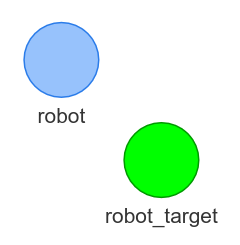
\includegraphics[width=0.7\textwidth]{figures/proposed_method/connecting_nodes/robot_to_target/robot_to_target}
    \end{subfigure}
    \begin{subfigure}{.3\textwidth}
    \centering
    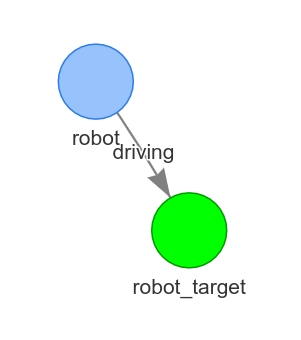
\includegraphics[width=0.9\textwidth]{figures/proposed_method/connecting_nodes/robot_to_target/robot_drive_target}
    \end{subfigure}
    \begin{subfigure}{.3\textwidth}
    \centering
    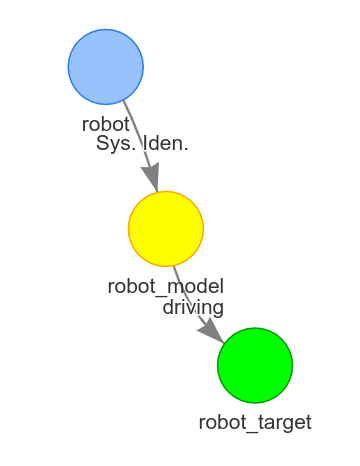
\includegraphics[width=\textwidth]{figures/proposed_method/connecting_nodes/robot_to_target/robot_iden_drive_target}
    \end{subfigure}
    \caption{\ac{hgraph} generated by the \ac{halgorithm} to drive the robot to a target configuration}%
    \label{fig:robot_drive_hgraph}
\end{figure}

The robot does not have a system model of itself, thus first system identification must be performed before it can drive to the specified target configuration. The \ac{kgraph} that will be discussed in \Cref{subsec:kgraph_definition} can suggest an action that includes a system model. In that case, system identification is not needed. The following figure displays successfully executing the hypothesis found in \Cref{fig:robot_drive_hgraph}.\bs

\begin{figure}[H]
    \centering
    \begin{subfigure}{.3\textwidth}
    \centering
    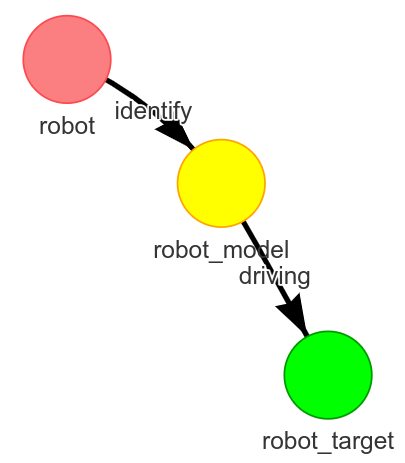
\includegraphics[width=0.9\textwidth]{figures/proposed_method/connecting_nodes/robot_to_target/execute_robot_to_target_1}
    \end{subfigure}
    \begin{subfigure}{.3\textwidth}
    \centering
    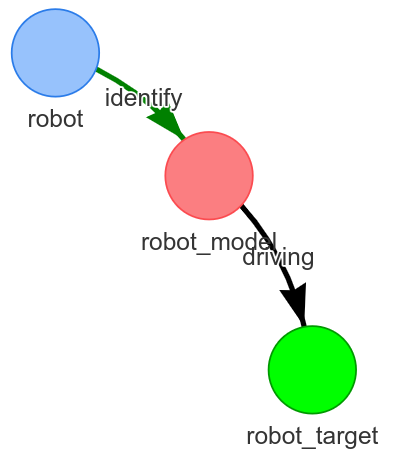
\includegraphics[width=0.9\textwidth]{figures/proposed_method/connecting_nodes/robot_to_target/execute_robot_to_target_2}
    \end{subfigure}
    \begin{subfigure}{.3\textwidth}
    \centering
    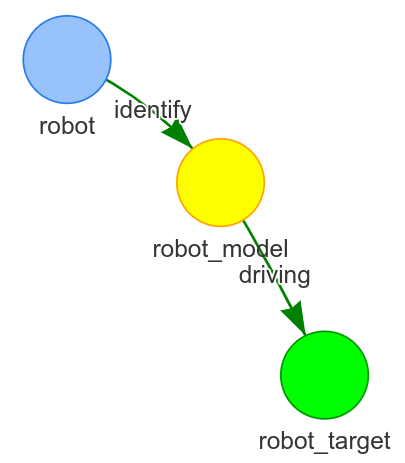
\includegraphics[width=0.9\textwidth]{figures/proposed_method/connecting_nodes/robot_to_target/execute_robot_to_target_3}
    \end{subfigure}
    \caption{Executing the hypothesis found in \Cref{fig:robot_drive_hgraph}.}
    \label{fig:execute_robot_to_target}
\end{figure}

Upcoming figure will display the hypothesis generated to push an object to a target position. Both generating a hypothesis and executing the hypothesis are intertwined, this is because certain information should first be collected from the environment before the full hypothesis can be generated. An example is the \textit{best\_push\_position} that can be found in \Cref{subfig:robot_push_7,subfig:robot_push_8,subfig:robot_push_9}. The \textit{best\_push\_position} can be found after manipulation planning for the pushing edge is completed. For motion planning a system model is required, thus the corresponding system identification edge should be completed before manipulation planning can start, and than the \textit{best\_push\_position} can be determined.\bs

\begin{figure}[H]
    \centering
    \begin{subfigure}{.3\textwidth}
    \centering
    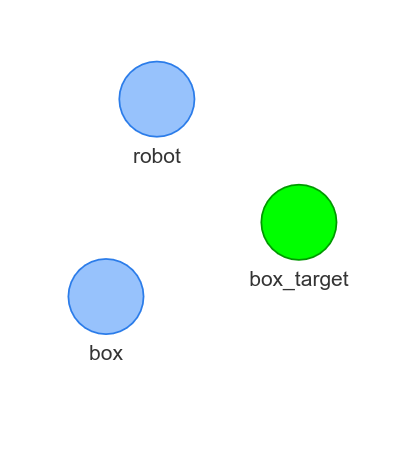
\includegraphics[width=0.8\textwidth]{figures/proposed_method/connecting_nodes/robot_push/robot_push_1}
    \caption{}
    \end{subfigure}
    \begin{subfigure}{.3\textwidth}
    \centering
    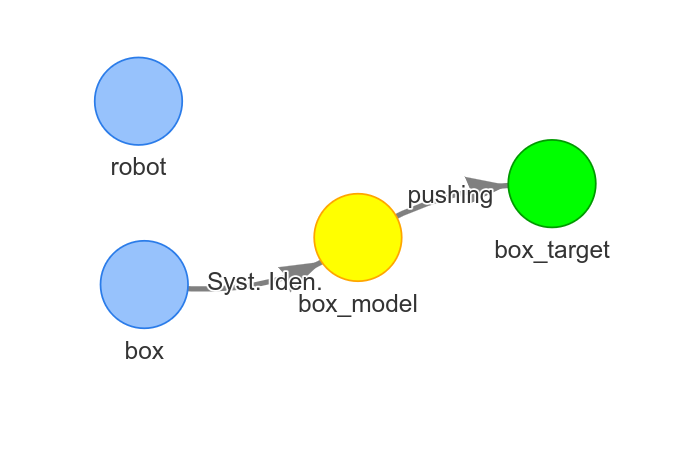
\includegraphics[width=1.1\textwidth]{figures/proposed_method/connecting_nodes/robot_push/robot_push_2}
    \caption{}\label{subfig:robot_push_2}
    \end{subfigure}
    \begin{subfigure}{.3\textwidth}
    \centering
    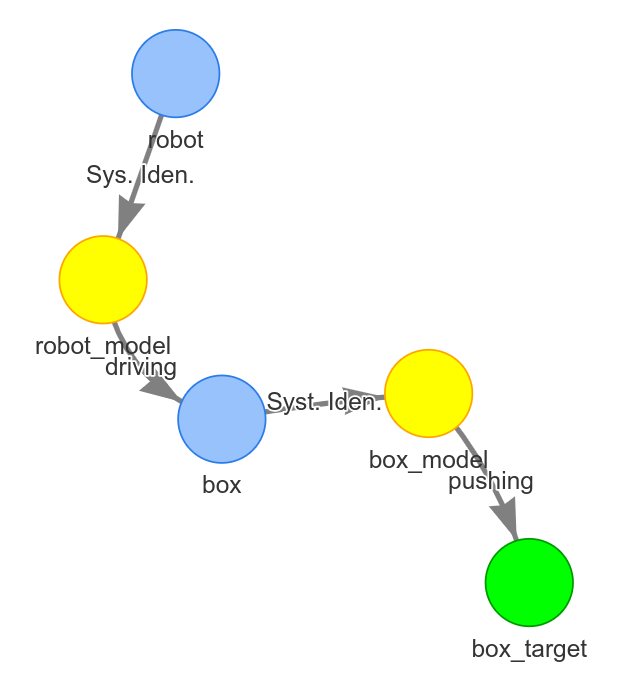
\includegraphics[width=1\textwidth]{figures/proposed_method/connecting_nodes/robot_push/robot_push_3}
    \caption{}\label{subfig:robot_push_3}
    \end{subfigure}

    \begin{subfigure}{.3\textwidth}
    \centering
    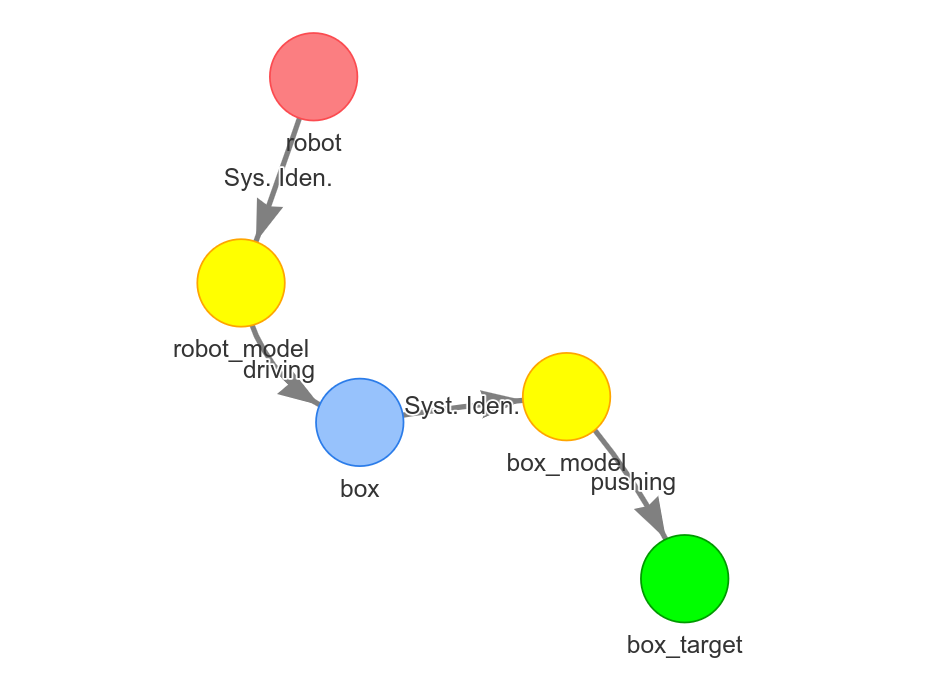
\includegraphics[width=1\textwidth]{figures/proposed_method/connecting_nodes/robot_push/robot_push_4}
    \caption{}\label{subfig:robot_push_4}
    \end{subfigure}
    \begin{subfigure}{.3\textwidth}
    \centering
    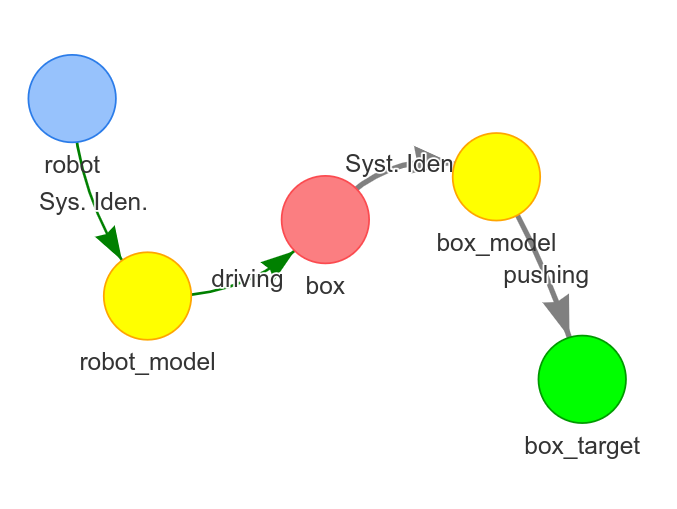
\includegraphics[width=1.05\textwidth]{figures/proposed_method/connecting_nodes/robot_push/robot_push_5}
    \caption{}\label{subfig:robot_push_5}
    \end{subfigure}
    \begin{subfigure}{.3\textwidth}
    \centering
    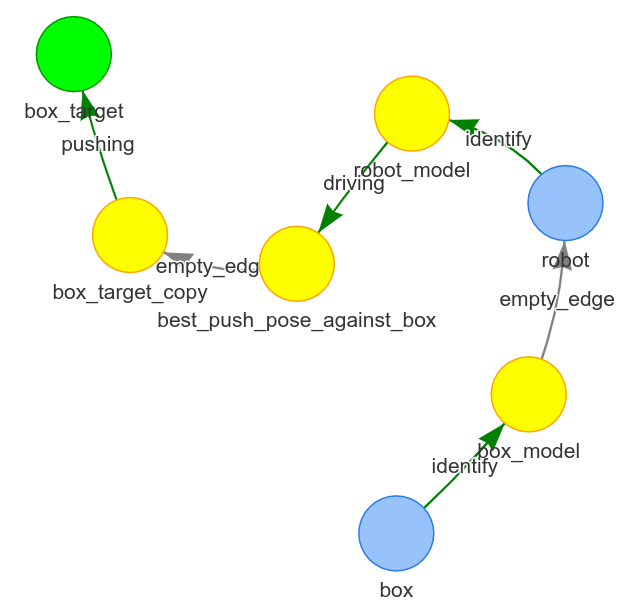
\includegraphics[width=1.05\textwidth]{figures/proposed_method/connecting_nodes/robot_push/robot_push_6}
    \caption{}\label{subfig:robot_push_6}
    \end{subfigure}

    \begin{subfigure}{.3\textwidth}
    \centering
    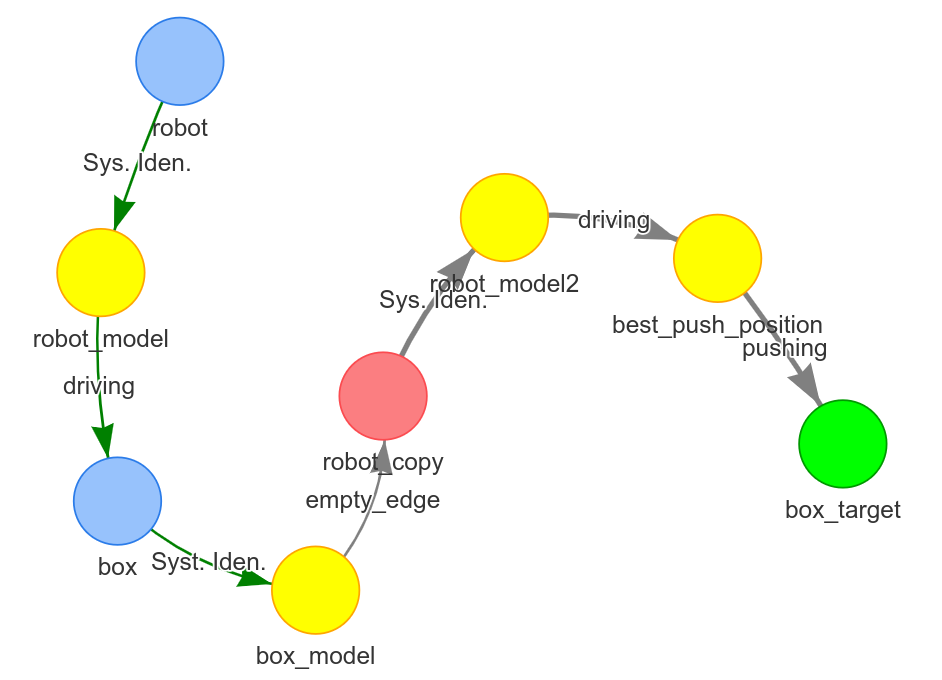
\includegraphics[width=1\textwidth]{figures/proposed_method/connecting_nodes/robot_push/robot_push_7}
    \caption{}\label{subfig:robot_push_7}
    \end{subfigure}
    \begin{subfigure}{.3\textwidth}
    \centering
    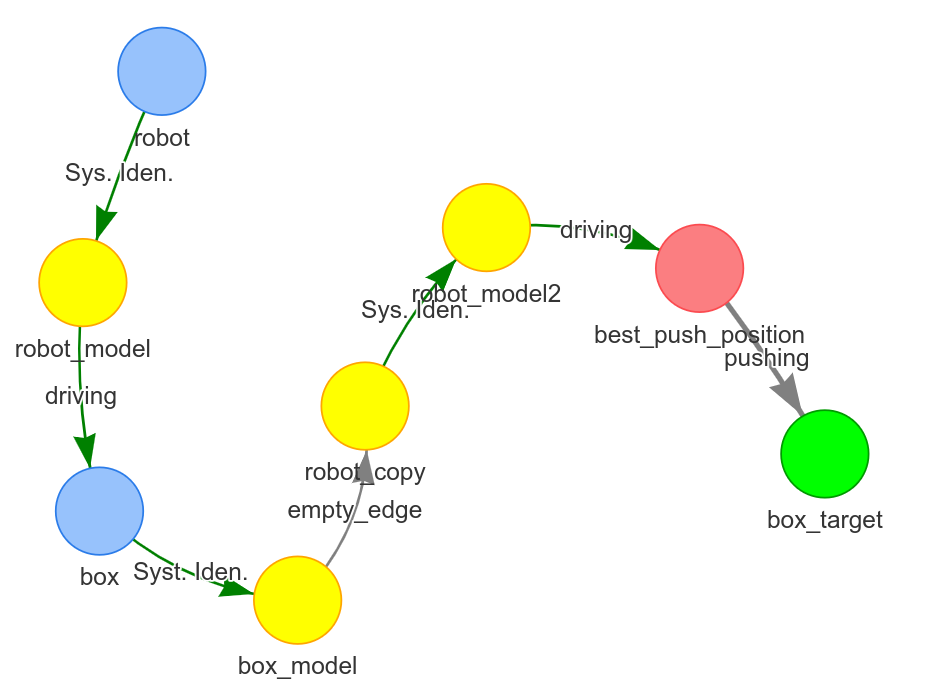
\includegraphics[width=1.05\textwidth]{figures/proposed_method/connecting_nodes/robot_push/robot_push_8}
    \caption{}\label{subfig:robot_push_8}
    \end{subfigure}
    \begin{subfigure}{.3\textwidth}
    \centering
    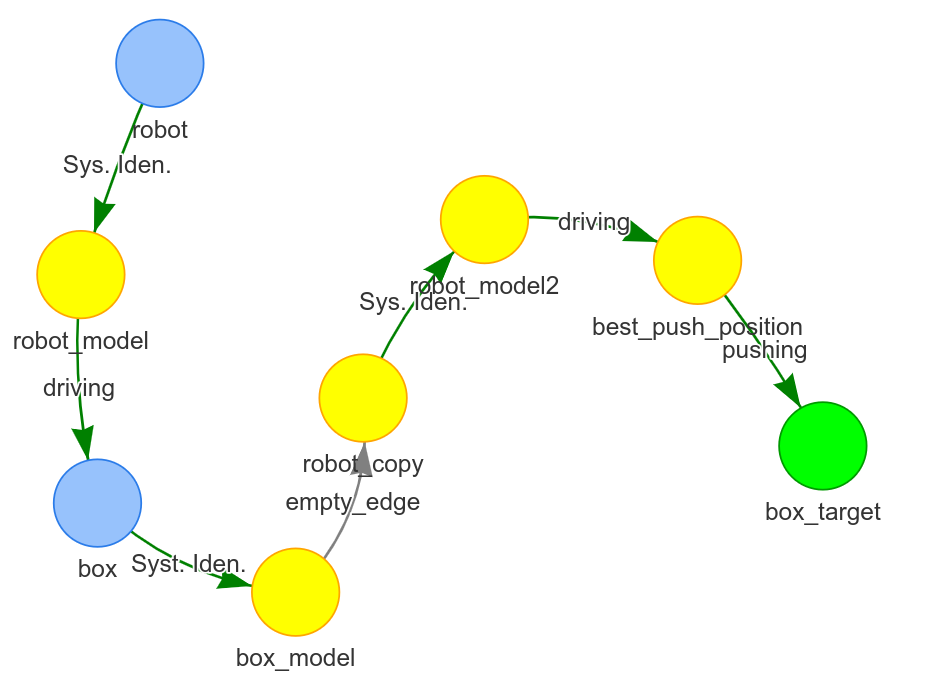
\includegraphics[width=1.05\textwidth]{figures/proposed_method/connecting_nodes/robot_push/robot_push_9}
    \caption{}\label{subfig:robot_push_9}
    \end{subfigure}
    \caption{\ac{hgraph} for pushing the green box to the target configuration}%
    \label{fig:robot_push_hgraph}
\end{figure}
Especially in \Cref{subfig:robot_push_2,subfig:robot_push_3} the backward search is clearly visible, the \ac{halgorithm} searches from target node to the robot node. \Cref{fig:robot_push_hgraph} is extensive because every necessary 

\todo{Corrado: bit unclear here, rewrite, IDK what's happenign here right}
steps is included whilst some could be skipped. First, identifying a system model for robot driving twice, if the system model created in edge Sys. Iden.~pointing toward node robot\_model is reused, then the edge Sys. Iden.~pointing toward robot\_model\_1 would be unnecessary. Second, if system models would already be available for driving and pushing, no single system identification edge would be required. A \textit{empty\_edge} can be seen in \Cref{subfig:robot_push_7,subfig:robot_push_8,subfig:robot_push_9}, the empty\_edge serves to connect a node to another node (box\_model to 

\todo{Corrado: why is there a robot copy?}
robot\_copy in \Cref{fig:robot_push_hgraph}). The empty\_edge can be traversed without execution, holds no controller, system model or status.\bs

\paragraph{Encountering a Blocked Path}%
During propagation of an action edge's status, motion or manipulation planning occurs. If an object is blocking the path, planning will detect it and the \ac{halgorithm} tries to free the path. In the next example the \ac{halgorithm} detects a blocking object and frees the path by pushing the blocking object to a new configuration, and can be visualized in \Cref{fig:blocking_obj_hgraph}.\bs

\begin{figure}[H]
    \centering
    \begin{subfigure}{.3\textwidth}
    \centering
    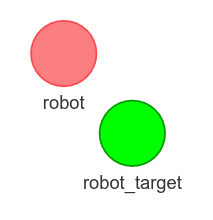
\includegraphics[width=0.6\textwidth]{figures/proposed_method/connecting_nodes/blocking_obj/blocking_obj_1}
    \caption{}
    \end{subfigure}
    \begin{subfigure}{.3\textwidth}
    \centering
    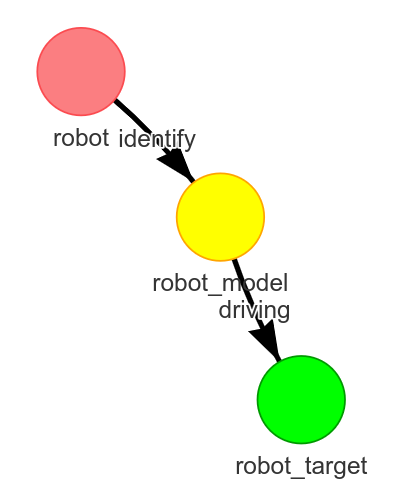
\includegraphics[width=0.9\textwidth]{figures/proposed_method/connecting_nodes/blocking_obj/blocking_obj_2}
    \caption{}\label{subfig:blocking_obj_2}
    \end{subfigure}
    \begin{subfigure}{.3\textwidth}
    \centering
    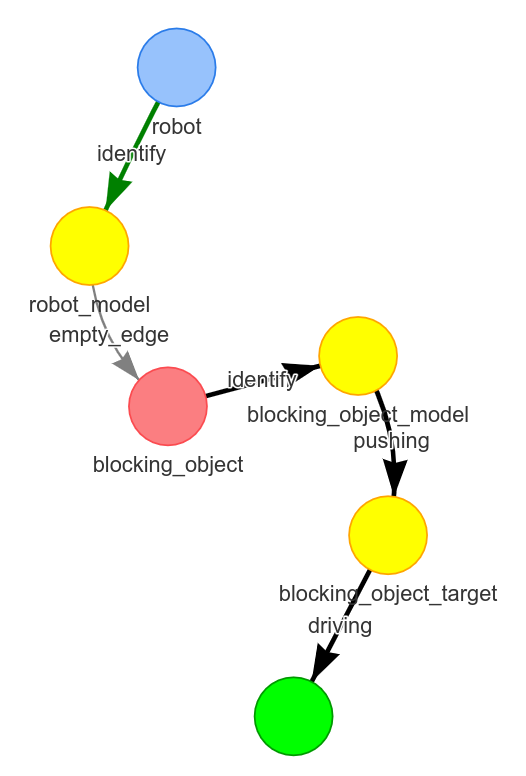
\includegraphics[width=\textwidth]{figures/proposed_method/connecting_nodes/blocking_obj/blocking_obj_3}
    \caption{}\label{subfig:blocking_obj_3}
    \end{subfigure}

    \begin{subfigure}{.3\textwidth}
    \centering
    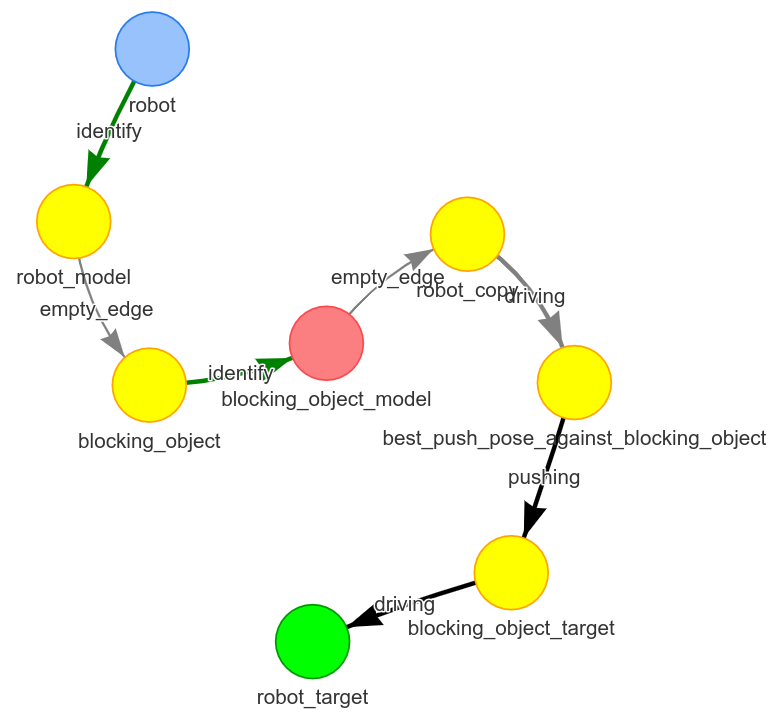
\includegraphics[width=1.291\textwidth]{figures/proposed_method/connecting_nodes/blocking_obj/blocking_obj_4}
    \caption{}\label{subfig:blocking_obj_4}
    \end{subfigure}
    \begin{subfigure}{.3\textwidth}
    \centering
    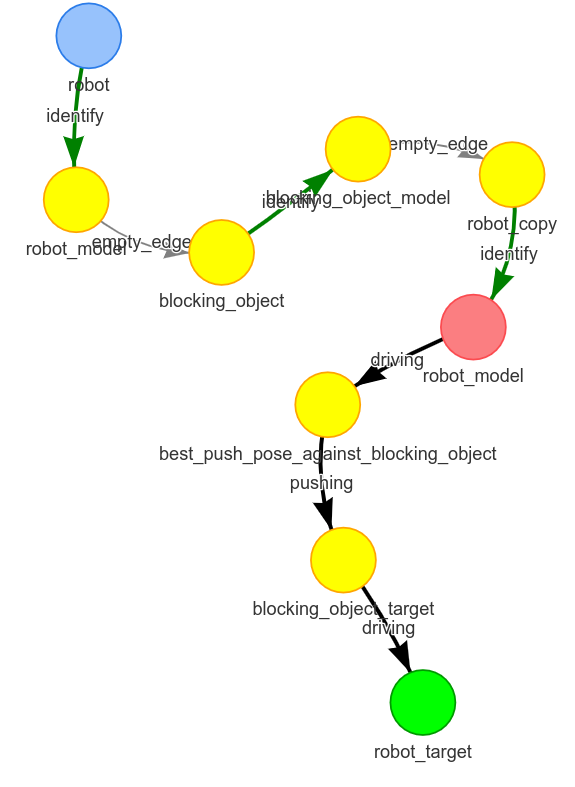
\includegraphics[width=\textwidth]{figures/proposed_method/connecting_nodes/blocking_obj/blocking_obj_5}
    \caption{}\label{subfig:blocking_obj_5}
    \end{subfigure}
    \begin{subfigure}{.3\textwidth}
    \centering
    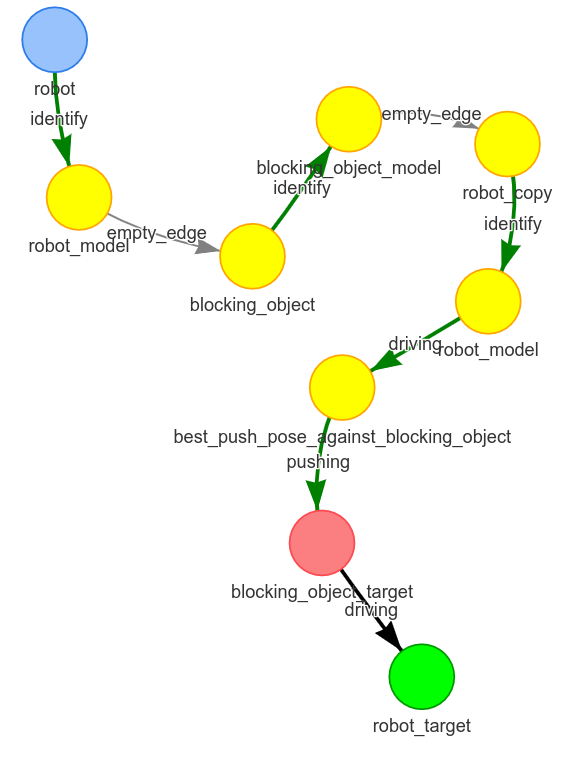
\includegraphics[width=\textwidth]{figures/proposed_method/connecting_nodes/blocking_obj/blocking_obj_6}
    \caption{}\label{subfig:blocking_obj_6}
    \end{subfigure}
    \caption{\ac{hgraph} for driving to target configuration and encountering a blocked path}%
    \label{fig:blocking_obj_hgraph}
\end{figure}

\paragraph{Encountering Failure}%
In the last example, \Cref{fig:failure_in_hgraph} the first hypothesis fails to complete and the \ac{halgorithm} tries to generate a new hypothesis that also fails to complete. Several faults and failures are modeled \todo{Corrado: where please ref?}, the \ac{halgorithm} response to faults and failure is the same. If during the propagation of an edge's status any kind of failure arises, the failed edge and corresponding edges are marked as failed. Equally during execution, if a fault is detected, the execution halts and the edge and corresponding edges are marked as \quotes{failed}, the procedure can be seen in \Cref{fig:failure_in_hgraph}.\bs

\begin{figure}[H]
    \centering
    \begin{subfigure}{.3\textwidth}
    \centering
    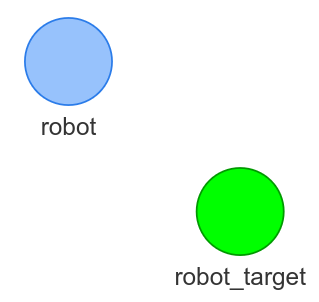
\includegraphics[width=0.8\textwidth]{figures/proposed_method/connecting_nodes/failure/fail_1}
    \end{subfigure}
    \begin{subfigure}{.3\textwidth}
    \centering
    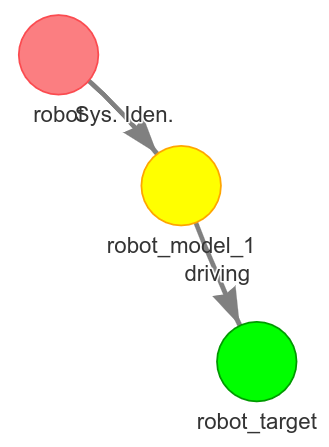
\includegraphics[width=1.05\textwidth]{figures/proposed_method/connecting_nodes/failure/fail_2}
    \end{subfigure}
    \begin{subfigure}{.3\textwidth}
    \centering
    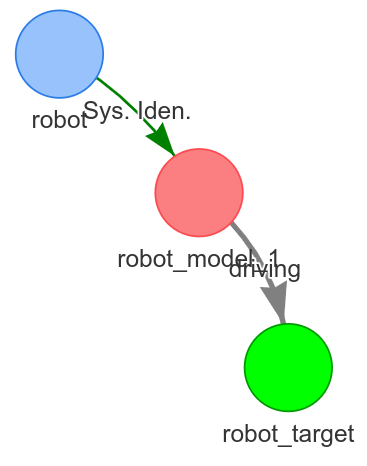
\includegraphics[width=\textwidth]{figures/proposed_method/connecting_nodes/failure/fail_3}
    \end{subfigure}

    \begin{subfigure}{.3\textwidth}
    \centering
    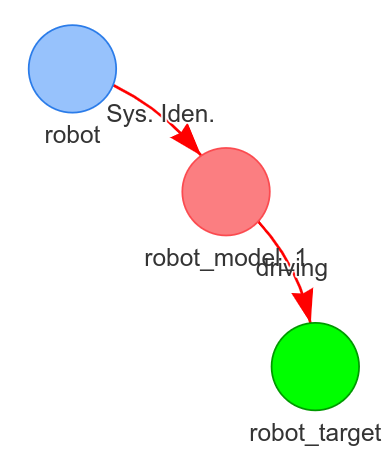
\includegraphics[width=1\textwidth]{figures/proposed_method/connecting_nodes/failure/fail_4}
    \end{subfigure}
    \begin{subfigure}{.3\textwidth}
    \centering
    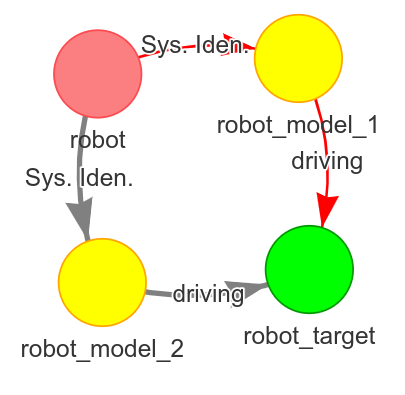
\includegraphics[width=1\textwidth]{figures/proposed_method/connecting_nodes/failure/fail_5}
    \end{subfigure}
    \begin{subfigure}{.3\textwidth}
    \centering
    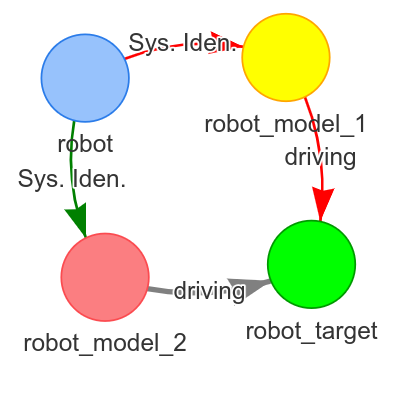
\includegraphics[width=1\textwidth]{figures/proposed_method/connecting_nodes/failure/fail_6}
    \end{subfigure}

    \begin{subfigure}{.3\textwidth}
    \centering
    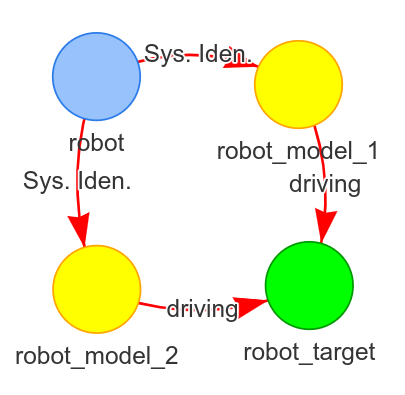
\includegraphics[width=1\textwidth]{figures/proposed_method/connecting_nodes/failure/fail_7}
    \end{subfigure}
    \hfill
    \caption{Executing two hypothesis, both failing to complete because a fault of failure emerged.}%
    \label{fig:failure_in_hgraph}
\end{figure}

In \Cref{fig:failure_in_hgraph} only two parameterizations of drive controller and system model were available. Thus after two failed hypothesis the \ac{halgorithm} concludes it cannot complete this task.\bs


What by now hopefully became clear to the reader is that the \ac{halgorithm} autonomously searches for hypotheses in the \ac{hgraph} to solve a task, one subtask at a time. The \ac{halgorithm} switches between the search and execution loop. Switching from the search loop toward the execution loop when a hypothesis is found, and switching back when a hypothesis is completed or an fault or failure occurred.\bs

The limited number of possible edge parameterization (every combination of a system identification method with a compatible control method) guarantees that the robot tries to complete a subtask, but concludes that it is unable to complete a subtask if all possible edges have failed.\bs

Recall the 3 topics (one, learning object dynamics, two the \ac{NAMO} problem and three nonprehensile push manipulation to target pose) that this thesis proposes to combine. The \ac{halgorithm} can solve \ac{NAMO} problems because the robot can drive toward target positions even if reaching such a position requires objects to be moved first. The proposed algorithm learns to classify objects by updating objects class from unknown to movable or obstacle. The \ac{halgorithm} can push objects to target positions by first identifying a system model and then pushing the object toward its target position. The system model that system identification yields is however of short use, it is only given to the corresponding action edge. In the next section, the edges that are executed will be reviewed and stored in a knowledge base, named the \acf{kgraph}. The \ac{kgraph} will suggest a parameterization based on the stored action reviews.\bs
